\appendix
\chapter{Non Linear Behavior of Horizontal Spring System under Vertical Load}

Fig~\ref{fig:Non_linear_system} below represents the system used for carrying out the study. The plot shown in fig~\ref{fig:Non_linear_system_plot} present the response of the system. The reaction is normalized by stiffness of the linear springs and the displacement are normalized by the natural lengths of the spring.

\begin{figure}[!htbp]
    \centering
    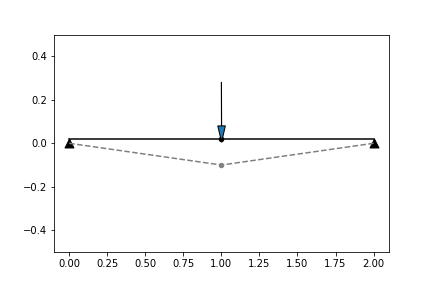
\includegraphics[width = 0.5\textwidth]{Figures/non_linear_spring_behavior.png}
    \caption{Spring system for Non-Linear behavior}
    \label{fig:Non_linear_system}
\end{figure}

\begin{figure}[!htbp]
    \centering
    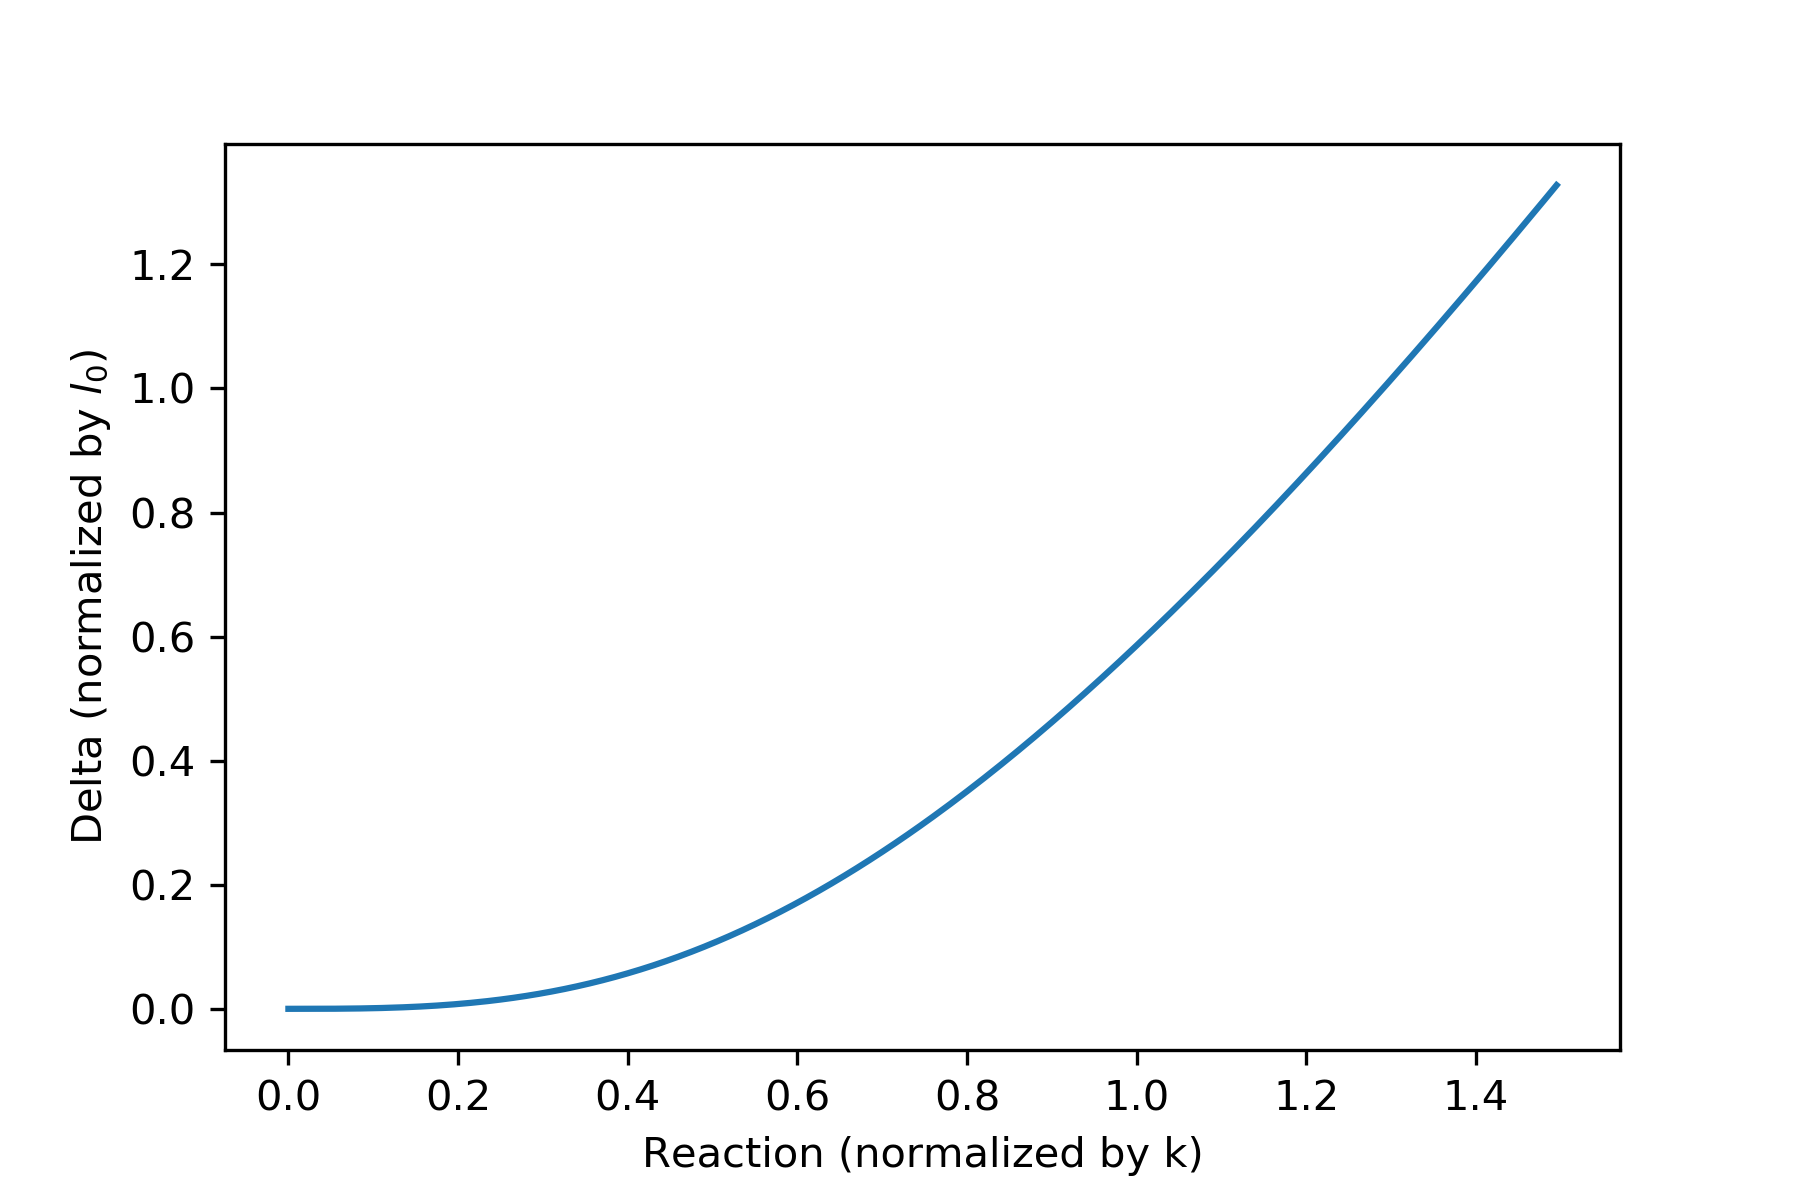
\includegraphics[width = 0.5\textwidth]{Figures/spring_response.png}
    \caption{Response of the Spring System}
    \label{fig:Non_linear_system_plot}
\end{figure}

As it can be seen from the response, initially the spring only offers second order reaction for small deflections at centre. With reference to the models presented in the project, this explains the crushing of the vertical springs at high loading since horizontal spring system offers no vertical reaction to the applied loading at the start. Adding body diagonals helps in distribution of the concentrated load and hence Model 3 is more stable performance under loading. 

